\documentclass{beamer}

\usetheme{Warsaw}    

\usepackage{listings}                                   
\usepackage{hyperref}
\usepackage{graphicx}                                 
\usepackage{tabularx}
\usepackage{microtype}
\usepackage[T1]{fontenc}
\usepackage[scaled]{beramono}

\usepackage{xcolor}

\newcommand\Small{\fontsize{5}{5.2}\selectfont}
\newcommand*\LSTfont{\Small\ttfamily\SetTracking{encoding=*}{-60}\lsstyle}

\hypersetup{colorlinks=color, linkcolor=black}
\definecolor{OliveGreen}{rgb}{0,0.6,0}
\graphicspath{{./images/}}
%
% Turn off beamer nav stuff...
%
\setbeamertemplate{navigation symbols}{}

%
% listings does not currently support clojure...here's an attempt I
% found in a discussion thread to add clojure support.
% For the moment, this results in decent looking code. I might switch
% to minted in the future.
%
\lstdefinelanguage{clojure}%
{morekeywords={*,*1,*2,*3,*agent*,*allow-unresolved-vars*,*assert*,*clojure-version*,*command-line-args*,%
*compile-files*,*compile-path*,*e,*err*,*file*,*flush-on-newline*,*in*,*macro-meta*,%
*math-context*,*ns*,*out*,*print-dup*,*print-length*,*print-level*,*print-meta*,*print-readably*,%
*read-eval*,*source-path*,*use-context-classloader*,*warn-on-reflection*,+,-,->,->>,..,/,:else,%
<,<=,=,==,>,>=,@,accessor,aclone,add-classpath,add-watch,agent,agent-errors,aget,alength,alias,%
all-ns,alter,alter-meta!,alter-var-root,amap,ancestors,and,apply,areduce,array-map,aset,%
aset-boolean,aset-byte,aset-char,aset-double,aset-float,aset-int,aset-long,aset-short,assert,%
assoc,assoc!,assoc-in,associative?,atom,await,await-for,await1,bases,bean,bigdec,bigint,binding,%
bit-and,bit-and-not,bit-clear,bit-flip,bit-not,bit-or,bit-set,bit-shift-left,bit-shift-right,%
bit-test,bit-xor,boolean,boolean-array,booleans,bound-fn,bound-fn*,butlast,byte,byte-array,%
bytes,cast,char,char-array,char-escape-string,char-name-string,char?,chars,chunk,chunk-append,%
chunk-buffer,chunk-cons,chunk-first,chunk-next,chunk-rest,chunked-seq?,class,class?,%
clear-agent-errors,clojure-version,coll?,comment,commute,comp,comparator,compare,compare-and-set!,%
compile,complement,concat,cond,condp,conj,conj!,cons,constantly,construct-proxy,contains?,count,%
counted?,create-ns,create-struct,cycle,dec,decimal?,declare,def,definline,defmacro,defmethod,%
defmulti,defn,defn-,defonce,defprotocol,defstruct,deftype,delay,delay?,deliver,deref,derive,%
descendants,destructure,disj,disj!,dissoc,dissoc!,distinct,distinct?,do,do-template,doall,doc,%
dorun,doseq,dosync,dotimes,doto,double,double-array,doubles,drop,drop-last,drop-while,empty,empty?,%
ensure,enumeration-seq,eval,even?,every?,false,false?,ffirst,file-seq,filter,finally,find,find-doc,%
find-ns,find-var,first,float,float-array,float?,floats,flush,fn,fn?,fnext,for,force,format,future,%
future-call,future-cancel,future-cancelled?,future-done?,future?,gen-class,gen-interface,gensym,%
get,get-in,get-method,get-proxy-class,get-thread-bindings,get-validator,hash,hash-map,hash-set,%
identical?,identity,if,if-let,if-not,ifn?,import,in-ns,inc,init-proxy,instance?,int,int-array,%
integer?,interleave,intern,interpose,into,into-array,ints,io!,isa?,iterate,iterator-seq,juxt,%
key,keys,keyword,keyword?,last,lazy-cat,lazy-seq,let,letfn,line-seq,list,list*,list?,load,load-file,%
load-reader,load-string,loaded-libs,locking,long,long-array,longs,loop,macroexpand,macroexpand-1,%
make-array,make-hierarchy,map,map?,mapcat,max,max-key,memfn,memoize,merge,merge-with,meta,%
method-sig,methods,min,min-key,mod,monitor-enter,monitor-exit,name,namespace,neg?,new,newline,%
next,nfirst,nil,nil?,nnext,not,not-any?,not-empty,not-every?,not=,ns,ns-aliases,ns-imports,%
ns-interns,ns-map,ns-name,ns-publics,ns-refers,ns-resolve,ns-unalias,ns-unmap,nth,nthnext,num,%
number?,odd?,or,parents,partial,partition,pcalls,peek,persistent!,pmap,pop,pop!,pop-thread-bindings,%
pos?,pr,pr-str,prefer-method,prefers,primitives-classnames,print,print-ctor,print-doc,print-dup,%
print-method,print-namespace-doc,print-simple,print-special-doc,print-str,printf,println,println-str,%
prn,prn-str,promise,proxy,proxy-call-with-super,proxy-mappings,proxy-name,proxy-super,%
push-thread-bindings,pvalues,quot,rand,rand-int,range,ratio?,rational?,rationalize,re-find,%
re-groups,re-matcher,re-matches,re-pattern,re-seq,read,read-line,read-string,recur,reduce,ref,%
ref-history-count,ref-max-history,ref-min-history,ref-set,refer,refer-clojure,reify,%
release-pending-sends,rem,remove,remove-method,remove-ns,remove-watch,repeat,repeatedly,%
replace,replicate,require,reset!,reset-meta!,resolve,rest,resultset-seq,reverse,reversible?,%
rseq,rsubseq,second,select-keys,send,send-off,seq,seq?,seque,sequence,sequential?,set,set!,%
set-validator!,set?,short,short-array,shorts,shutdown-agents,slurp,some,sort,sort-by,sorted-map,%
sorted-map-by,sorted-set,sorted-set-by,sorted?,special-form-anchor,special-symbol?,split-at,%
split-with,str,stream?,string?,struct,struct-map,subs,subseq,subvec,supers,swap!,symbol,symbol?,%
sync,syntax-symbol-anchor,take,take-last,take-nth,take-while,test,the-ns,throw,time,to-array,%
to-array-2d,trampoline,transient,tree-seq,true,true?,try,type,unchecked-add,unchecked-dec,%
unchecked-divide,unchecked-inc,unchecked-multiply,unchecked-negate,unchecked-remainder,%
unchecked-subtract,underive,unquote,unquote-splicing,update-in,update-proxy,use,val,vals,%
var,var-get,var-set,var?,vary-meta,vec,vector,vector?,when,when-first,when-let,when-not,%
while,with-bindings,with-bindings*,with-in-str,with-loading-context,with-local-vars,%
with-meta,with-open,with-out-str,with-precision,xml-seq,zero?,zipmap
},%
   sensitive,% ???
   alsodigit=-,%
   morecomment=[l];,%
   morestring=[b]"%
  }[keywords,comments,strings]%

\lstset{
%  frame=tb,
  language=clojure,
% showstringspaces=false,
%  keepspaces=true
%  columns=fullflexible,
%  basicstyle={\LSTfont},
  numbers=none,
  numberstyle=\tiny\color{gray},
  keywordstyle=\color{blue},
  commentstyle=\color{orange},
  stringstyle=\color{OliveGreen},
%  breaklines=false,
%  breakatwhitespace=false
  tabsize=2
}


\begin{document}


\begin{frame}
  \frametitle{Clojure Intro}
  \center{
    
\includegraphics[scale=.40]{Clojure-Logo}
  }

  June 2014

\end{frame}

\frame{
  \frametitle{A Brief History of Lisp}
  \begin{columns}
    \begin{column}{.49\textwidth}
      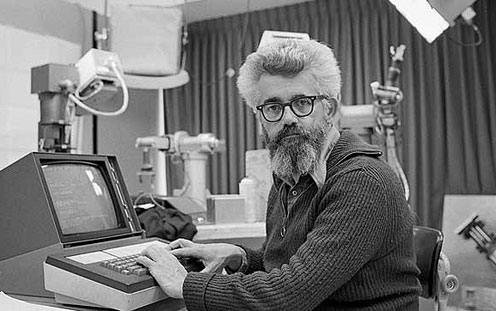
\includegraphics[scale=.60]{john-mccarthy}
    \end{column}
    \begin{column}{.49\textwidth}
      \itemize{
      \item John McCarthy 1958
      }
    \end{column}
  \end{columns}
}

\frame{
  \frametitle{Notable Attributes of the Original Lisp}
  \begin{itemize}
    \item Conditionals
    \item A function type
    \item Recursion
    \item Variables as pointers
    \item Garbage Collection
  \end{itemize}
}


\frame{
  \frametitle{Scheme 1975-1980}
  \begin{columns}
    \begin{column}{.49\textwidth}
      Guy Steele
      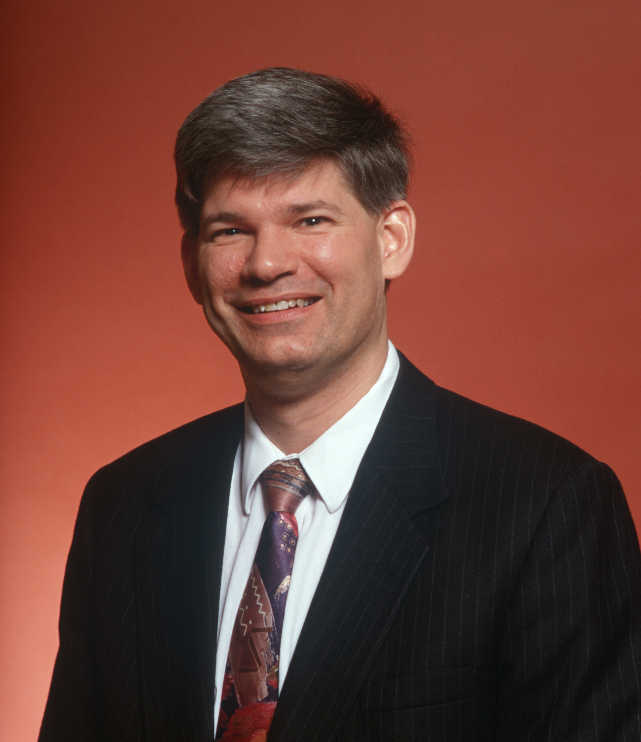
\includegraphics[scale=.25]{guy-steele}
    \end{column}
    \begin{column}{.49\textwidth}
      Gerald Sussman
      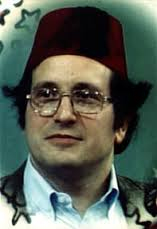
\includegraphics[scale=.80]{gerald-sussman}
    \end{column}
  \end{columns}
}

\frame{
  \frametitle{Racket - Mid 1990s}
}

\frame{
  \frametitle{Clojure 2007}
  \center{
    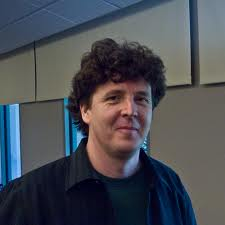
\includegraphics[scale=.80]{rich-hickey}
  }
  Rich Hickey
}

\frame{
  \frametitle{Clojure Distinguishing Characteristics}
  \begin{itemize}
    \item Immutability is the Default 
    \pause
    \item Unified Sequences 
    \pause
    \item Concurrency Support 
    \pause
    \item Embraces Java 
    \pause
  \end{itemize}
}

\begin{frame}
  \frametitle{Clojure Syntax}
  \begin{tabularx}{\textwidth}{ |X|X| }
  \hline
  Form & (fn-name fn-arg...)  \\
  \hline
  Vector & []  \\
  \hline
  Map(hash) &    \{\}  \\
  \hline
  Set &    \#\{\} \\
  \hline
  Keyword(symbol) & :some-keyword  \\
  \hline
  \end{tabularx}
\end{frame}

\begin{frame}
  \frametitle{Functions}
  \itemize{
    \item show func with optional declarations
  }
\end{frame}

\begin{frame}
  \frametitle{Control Flow Primitives}
\end{frame}

\begin{frame}
  \frametitle{Sequences}
  \itemize {
  \item Referred to as Seqs (pronouced seeks)
  \item Unified interface for maps, lists, trees, and arrays  
  }
\end{frame}

\begin{frame}
  \frametitle{vars and refs}
\end{frame}

\begin{frame}
  \frametitle{namespaces}
  \itemize{
  \item clojure.lang.Namespace
  \item current accessible via nsy
  }  
\end{frame}

\begin{frame}
  \frametitle{Naming Conventions}
  \itemize{
  \item ear muffs
  }  
\end{frame}

\begin{frame}
  \frametitle{Java Interop}
  
  \itemize{
    \item javadoc
    \item memfn
    \item dot special form
    \item bean
  }
\end{frame}

\begin{frame}
  \frametitle{Code Samples} 
  \lstinputlisting[language=clojure]{src/factory.clj} 

\end{frame}  

\end{document}
